\documentclass[12pt]{article}
\usepackage[utf8]{inputenc}
\usepackage[T1]{fontenc}
\usepackage[a4paper, left=2.4cm, right=2.4cm, top=2cm, bottom=2cm, nomarginpar]{geometry}
\usepackage{amsmath, algorithm, pgfplots, pgf, pdfpages, amsfonts, amssymb, stmaryrd, enumitem,graphicx, algpseudocode, setspace, listings, courier, color, caption, centernot, hyperref, lstautogobble, zi4, mathtools, lmodern, colortbl, array, multicol, fancyhdr, lastpage, svg}
\usepackage{booktabs}
\hypersetup{
    pdftitle={CE204_FP1_G6},
    pdftoolbar=true,        % show Acrobat’s toolbar?
    pdfmenubar=true,        % show Acrobat’s menu?
    pdfauthor={Muhammet Yağcıoğlu},
    pdfsubject={CE204_FP_RPs},
    pdfcreator={Muhammet Yağcıoğlu},   % creator of the document
    pdfproducer={Muhammet Yağcıoğlu}, % producer of the document
    colorlinks,
    linkcolor={black},
    citecolor={black},
    urlcolor={blue!80!black}
}
\usepackage[noblocks]{authblk}
\usepackage[version=4]{mhchem}
\usepackage[export]{adjustbox}
\usepackage{eso-pic} % Required for absolute positioning
\graphicspath{ {./images/} }
\usetikzlibrary{patterns}
\usepackage{tikz-3dplot}
\usepackage[version=4]{mhchem}
\usepackage[export]{adjustbox}
\usepgfplotslibrary{groupplots}
\usepackage{xcolor}
\usepackage[absolute,overlay]{textpos}
\usepackage{ragged2e}
\usepackage{xcolor}
\usepackage{amsthm}
\usepackage{tikz}




%----------compiler settings---------
\setlength{\parindent}{0pt}
\everymath{\displaystyle}
\onehalfspacing

%-----------colors----------
\pgfplotsset{compat=1.18}
\definecolor{bluekeywords}{rgb}{0.13, 0.13, 1}
\definecolor{greencomments}{rgb}{0, 0.5, 0}
\definecolor{redstrings}{rgb}{0.9, 0, 0}
\definecolor{graynumbers}{rgb}{0.5, 0.5, 0.5}
\definecolor{bronze}{rgb}{0.82, 0.41, 0.12}
\definecolor{crimson}{rgb}{0.86, 0.08, 0.24}
\definecolor{brown(web)}{rgb}{0.65, 0.16, 0.16}
\definecolor{darkspringgreen}{rgb}{0.16, 0.32, 0.75}
\definecolor{blue(ncs)}{rgb}{0.0, 0.53, 0.74}
\definecolor{amber}{rgb}{1.0, 0.49, 0.0}
\definecolor{cadmiumgreen}{rgb}{0.0, 0.42, 0.24}




%-------code frame-----------
\lstset{
    autogobble,
    columns=fullflexible,
    showspaces=false,
    showtabs=false,
    breaklines=true,
    showstringspaces=false,
    breakatwhitespace=true,
    escapeinside={(*@}{@*)},
    commentstyle=\color{greencomments},
    keywordstyle=\color{bluekeywords},
    stringstyle=\color{redstrings},
    numberstyle=\color{graynumbers},
    basicstyle=\ttfamily\footnotesize,
    frame=l,
    framesep=12pt,
    xleftmargin=12pt,
    tabsize=4,
    captionpos=b
}



\lstdefinelanguage{myMMA}{
keywords={SetDirectory, NotebookDirectory, Exp, IdentityMatrix, Eigenvalues, 
ListPlot, PlotRange, PlotStyle, Directive, PointSize, AspectRatio, Blue, Graphics, Line, 
Manipulate, Show, Sqrt, UniformDistribution, GammaDistribution, BetaDistribution, 
Nintegrate, For, DataRange, AxesLabel, PlotLabel, Transpose, Export, Plot, Append, Infinity},
keywordstyle=\color{black},
commentstyle=\color{gray}, 
identifierstyle=\color{blue},
sensitive=false,
comment=[l]{(*},
morecomment=[s]{/*}{*/},
morestring=[b]',
morestring=[b]"
}






%-----gauss declare---------
\pgfmathdeclarefunction{gauss}{2}{%
  \pgfmathparse{1/(#2*sqrt(2*pi)) * exp(-((x-#1)^2)/(2*#2^2))}%
}
\usetikzlibrary{arrows.meta, decorations.markings}
\pgfplotsset{compat=1.17}







%--------------page numbering------------
\fancyfoot[R]{page \thepage\ of \textcolor{bronze}{\pageref{LastPage}}}
\fancyhead[R]{Group 6}



%-------------qframe settings---------------

\usepackage[framemethod=TikZ]{mdframed}
\newmdenv[%
    skipabove=1em, % space above the frame
    skipbelow=1em, % space below the frame
    linewidth=1pt, % width of the frame lines
    linecolor=gray!80, % color of the frame lines
    backgroundcolor=gray!9, % background color inside the frame
    roundcorner=5pt, % radius of the rounded corners
    innerleftmargin=1em, % margin within the frame at the left
    innerrightmargin=1em, % margin within the frame at the right
    innertopmargin=0.5em, % margin within the frame at the top
    innerbottommargin=0.5em % margin within the frame at the bottom
]{qframe}

\newenvironment{q}
{
    \begin{qframe}
    \noindent\textit{\textbf{Problem Statement:}}
    \par\smallskip
}
{
    \end{qframe}
}





%-------------ANSWER TAG---------------
\newcommand{\AnswerTag}{\hfill 
\begin{tikzpicture} \fill[black] (0.35cm,0) -- (0,0.175cm) -- (0.35cm,0.35cm) -- cycle;\end{tikzpicture}}



%-------Theorem and another question frames----------
\newenvironment{theorem}{\begin{mdframed}\textbf{Theorem.}}{\end{mdframed}}

%usage: \begin{theorem}

\newenvironment{question}{\begin{mdframed}\textbf{Question.}}{\end{mdframed}}

%usage: %usage: \begin{question}
\fancyhead[L]{CE 224 Mechanics of Materials, Fall 2023, Homework-3 }
\title{\vspace{-1cm}CE 224 - HW3}
\author{Muhammet Yağcıoğlu - 290204042}
\usepackage{hyperref} 
\begin{document}
\maketitle\thispagestyle{fancy}
\pagestyle{fancy}
\tableofcontents
\newpage



\section*{Question 1}
\addcontentsline{toc}{section}{Question 1}
\begin{q}
1. Determine the maximum tensile stress and maximum compressive stress due to the load acting on the simple beam shown in figure.

Data are as follows:

\(P=6.2 \mathrm{kN}, L=3.2 \mathrm{~m}, \mathrm{~d}=1.25 \mathrm{~m}, \mathrm{~b}=80 \mathrm{~mm}, \mathrm{t}=25 \mathrm{~mm}, \mathrm{~h}=120 \mathrm{~mm}\), and \(h_1=90 \mathrm{~mm}\).

\end{q}


\begin{figure}[!ht]
    \centering
    \resizebox{0.7\textwidth}{!}{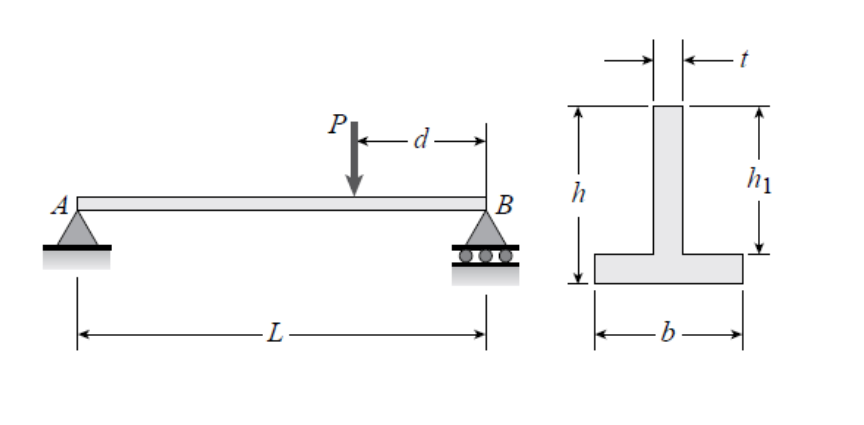
\includegraphics{image.png}}
    \caption{}
    \label{fig:enter-label}
\end{figure}

Let \( P = 6.2 \, \text{kN} \), \( L = 3.2 \, \text{m} \), \( d = 1.25 \, \text{m} \), \( b = 80 \, \text{mm} \), \( t = 25 \, \text{mm} \), \( h = 120 \, \text{mm} \), and \( h_1 = 90 \, \text{mm} \) the given parameters of the problem. The cross-sectional area of the beam is composed of two rectangles, the upper rectangle with dimensions \( t \times b \) and the lower rectangle with dimensions \( (h - h_1) \times b \). To calculate the centroid (neutral axis, $NA$) of this composite section, apply the theorem of composite areas (Hibbeler, R.C. (2013). Mechanics of Materials (9th ed.). [page 789, A.1, [Centroid od an area].). The distance of the centroid from the base, \( c_2 \), is
\[
c_2 = \frac{b \cdot \frac{(h - h_1)^2}{2} + h_1 \cdot t \cdot \left( h - h_1 + \frac{h_1}{2} \right)}{b \cdot (h - h_1) + h_1 \cdot t}
\]
\[= \frac{0.080 \cdot \frac{(0.120 - 0.090)^2}{2} + 0.090 \cdot 0.025 \cdot \left( 0.120 - 0.090 + \frac{0.090}{2} \right)}{0.080 \cdot (0.120 - 0.090) + 0.090 \cdot 0.025} = 0.044032 \, \text{m} = 44.032 \mathrm{~mm} \]
Further, \( c_1 = h - c_2 \) is the distance of the centroid from the opposite face.
\[c_2=75.968 \mathrm{~mm}\]

To determine the moment of inertia (I) about the $NA$, use the parallel axis theorem (Huygens–Steiner theorem) for each rectangle:

\[
I = b \cdot \frac{(h - h_1)^3}{12} + b \cdot (h - h_1) \cdot \left[ c_2 - \left( \frac{h - h_1}{2} \right) \right]^2 + \frac{t \cdot h_1^3}{12} + t \cdot h_1 \cdot \left( c_1 - \frac{h_1}{2} \right)^2 = 5.879 \times 10^{-6} \mathrm{~m}^4
\]

The maximum bending moment (\( M_{\text{max}} \)) in the beam occurs at the point of application of the load \( P \). Using the principles of static equilibrium, \( M_{\text{max}} \) is given by
\(R_A + R_B = P\), \(R_B \cdot L = P \cdot d \implies R_B = \frac{P \cdot d}{L}\) ,\(M_{\text{max}} = R_A \cdot d, \, R_A = P - R_B = P - \frac{P \cdot d}{L} \), \(M_{\text{max}} = \left( P - \frac{P \cdot d}{L} \right) \cdot d = P \cdot d - \frac{P \cdot d^2}{L} \implies M_{\text{max}} = \frac{P \cdot d}{L} \cdot (L - d)\):

\[
M_{\text{max}} = \frac{P \cdot d}{L} \cdot (L - d) = 4.72 \mathrm{kN} \cdot \mathrm{m}
\]


The maximum tensile stress (\( \sigma_t \)) and compressive stress (\( \sigma_c \)) are found using the flexure formula:

\[
\sigma_t = \frac{M_{\text{max}} \cdot c_2}{I}, \quad \sigma_c = \frac{M_{\text{max}} \cdot c_1}{I}
\]

Substitute the previously calculated values of \( M_{\text{max}} \), \( c_1 \), \( c_2 \), and \( I \) to find \( \sigma_t \) and \( \sigma_c \).


\[\sigma_c=\frac{M_{\max } c_1}{I}=61 \mathrm{MPa} \quad \sigma_t=\frac{M_{\max } c_2}{I}=35.4 \mathrm{MPa}\]

\AnswerTag













\vfill
\begin{flushright}
\textbf{ans.} \(\sigma_c=61 \mathrm{MPa}, \sigma_t=35.4 \mathrm{MPa}\)
\end{flushright}

\newpage
\section*{Question 2}
\addcontentsline{toc}{section}{Question 2}
\begin{q}
2. A cantilever beam \(A B\) of isosceles trapezoidal cross section has length \(L=0.8 \mathrm{~m}\), dimensions \(b_1=\) \(80 \mathrm{~mm}, b_2=90 \mathrm{~mm}\), and height \(h=110 \mathrm{~mm}\). The beam is made of brass weighing \(85 \mathrm{kN} / \mathrm{m}^3\).
(a) Determine the maximum tensile stress and maximum compressive stress due to the beam's own weight.
(b) If the width \(b_1\) is doubled, what happens to the stresses?
(c) If the height \(h\) is doubled, what happens to the stresses?
\end{q}
\begin{figure}[!ht]
    \centering
    \resizebox{0.7\textwidth}{!}{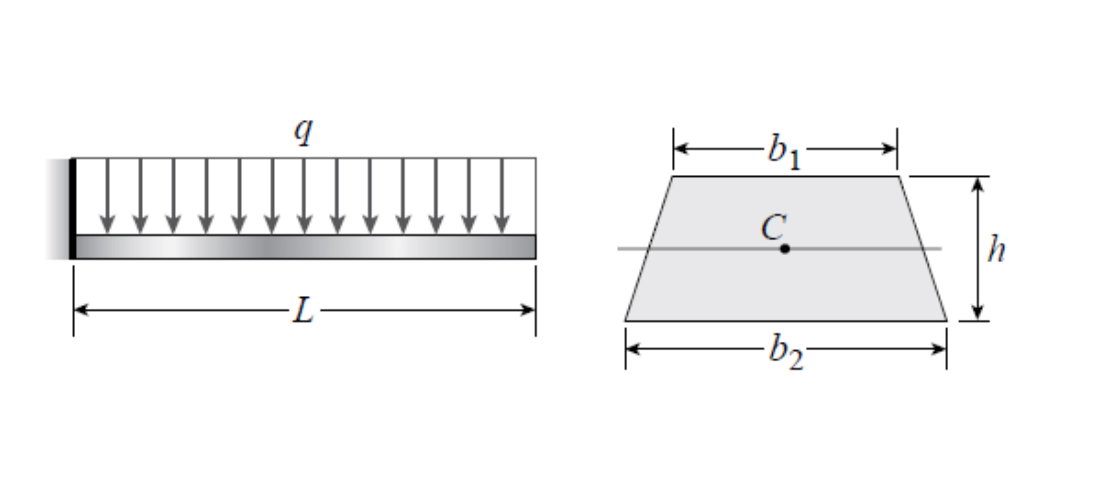
\includegraphics{image2.png}}
    \caption{}
    \label{fig:enter-label}
\end{figure}


\subsection*{Part a}


Let \( L = 0.8 \, \text{m} \), \( \gamma = 85 \, \text{kN/m}^3 \), \( b_1 = 80 \, \text{mm} \), \( b_2 = 90 \, \text{mm} \), and \( h = 110 \, \text{mm} \) the physical dimensions and material property of the cantilever beam in question. First, consider the area \( A \) of the trapezoidal cross-section. This is given by \( A = h(b_1 + b_2)/2 \). Substituting the values, \( A = \left(0.11 \times (0.08 + 0.09)\right)/2 \, \text{m}^2 = 0.00935 \, \text{m}^2 =  9.35 \times 10^3 \mathrm{~mm}^2\). The uniform load \( q \) due to the weight of the beam is \( q = \gamma A \). For brass with \( \gamma = 85 \, \text{kN/m}^3 \), the load is \( q = 85 \times 10^3 \times 0.00935 \, \text{N/m} = 794.75 \, \text{N/m} = 7.9475 \times 10^2 \, \text{N/m} \). The maximum bending moment \( M_{\text{max}} \) for a cantilever beam under uniformly distributed load is \( M_{\text{max}} = q L^2 /2 \). Substituting \( q = 794.75 \, \text{N/m} \) and \( L = 0.8 \, \text{m} \), we find \( M_{\text{max}} = \left(794.75 \times 0.8^2\right)/2 \,\, \text{Nm} = 254.32 \mathrm{~N} \cdot \mathrm{m}\). The moment of inertia \( I_C \) of the trapezoidal section about its neutral axis is calculated using the formula \href{formula}{\url{https://www.efunda.com/math/areas/IsosTrapezoid.cfm}} and Formulas for Stress and Strain Book by Ali M. Sadegh, Richard G. Budynas, and Warren C. Young, TABLE A.1, page 806. \( I_C = \frac{h^3(b_1^2 + 4b_1b_2 + b_2^2)}{36(b_1 + b_2)} \). Inserting the given dimensions yields \( I_C = \left[0.11^3(0.08^2 + 4 \times 0.08 \times 0.09 + 0.09^2)\right]/\left(36 \times (0.08 + 0.09)\right) \, \text{m}^4 =9.417 \times 10^6 \mathrm{~mm}^4 .\) Thus \(y_{\mathrm{bar}}=\frac{h\left(2 b_1+b_2\right)}{3\left(b_1+b_2\right)}=53.922 \mathrm{~mm}\) and then the maximum tensile stress \( \sigma_t \) and the maximum compressive stress \( \sigma_c \) is computed as

\[
\sigma_t = \frac{M_{\text{max}}(h - y_{\text{bar}})}{I_C} = \frac{254.32 \times (0.11 - 0.053922)}{9.417 \times 10^6} \, \text{Pa} = 1.514 \, \text{MPa},
\]
\[
\sigma_c = \frac{M_{\text{max}} y_{\text{bar}}}{I_C} = \frac{254.32 \times 0.053922}{9.417 \times 10^6} \, \text{Pa} =1.456 \, \text{MPa}.
\]

\subsection*{Part b}

We redefine the width \(b_1\) as \(b_1 = 2 \times 80 \, \text{mm} = 160 \, \text{mm}\). In turn, this change affects the beam's ability to support weight and distribute stress by changing the cross-section's shape. The area \(A\) of the modified trapezoidal cross-section becomes \[ A = \frac{1}{2} h (b_1 + b_2) = \frac{1}{2} \times 110 \, \text{mm} \times (160 \, \text{mm} + 90 \, \text{mm}) = 1.375 \times 10^4 \, \text{mm}^2. \] The uniform load \(q\) is recalculated as \( q = \gamma A = 85 \times 10^3 \, \text{N/m}^3 \times 1.375 \times 10^4 \, \text{mm}^2 \times 10^{-6} \, \text{m}^2/\text{mm}^2 = 1.169 \times 10^3 \, \text{N/m}. \) The maximum bending moment \(M_{\text{max}}\) for the cantilever beam is now \[ M_{\text{max}} = \frac{q L^2}{2} = \frac{1.169 \times 10^3 \, \text{N/m} \times (0.8 \, \text{m})^2}{2} = 374 \, \text{N} \cdot \text{m}. \] The centroid \(y_{\text{bar}}\) is now \[ y_{\text{bar}} = \frac{h(2b_1 + b_2)}{3(b_1 + b_2)} = \frac{110 \, \text{mm} \times (2 \times 160 \, \text{mm} + 90 \, \text{mm})}{3 \times (160 \, \text{mm} + 90 \, \text{mm})} = 60.133 \, \text{mm}. \] The moment of inertia \(I\) for the trapezoidal section about the neutral axis is now \[ I = h^3 \frac{(b_1^2 + 4b_1b_2 + b_2^2)}{36(b_1 + b_2)} = (110 \, \text{mm})^3 \times\frac{((160 \, \text{mm})^2 + 4 \times 160 \, \text{mm} \times 90 \, \text{mm} + (90 \, \text{mm})^2)}{36 \times (160 \, \text{mm} + 90 \, \text{mm})} = 1.35 \times 10^7 \, \text{mm}^4. \] Thus, the maximum tensile stress \( \sigma_t \) and compressive stress \( \sigma_c \) are now

\[ \sigma_t = \frac{M_{\text{max}}(h - y_{\text{bar}})}{I} = \frac{374 \, \text{N} \cdot \text{m} \times (110 \, \text{mm} - 60.133 \, \text{mm})}{1.35 \times 10^7 \, \text{mm}^4} = 1.381 \, \text{MPa}, \]
\[ \sigma_c = \frac{M_{\text{max}} y_{\text{bar}}}{I} = \frac{374 \, \text{N} \cdot \text{m} \times 60.133 \, \text{mm}}{1.35 \times 10^7 \, \text{mm}^4} = 1.666 \, \text{MPa}. \]
\AnswerTag



\subsection*{Part c}
We redefine the height \(h\) as \(h = 2 \times 110 \, \text{mm} = 220 \, \text{mm}\). The area \(A\) of the trapezoidal cross-section, now \[ A = \frac{1}{2} h (b_1 + b_2) = \frac{1}{2} \times 220 \, \text{mm} \times (80 \, \text{mm} + 90 \, \text{mm}) = 1.87 \times 10^4 \, \text{mm}^2. \] The uniform load \(q\) is now \( q = \gamma A = 85 \times 10^3 \, \text{N/m}^3 \times 1.87 \times 10^4 \, \text{mm}^2 \times 10^{-6} \, \text{m}^2/\text{mm}^2 = 1.589 \times 10^3 \, \text{N/m}. \) The maximum bending moment \(M_{\text{max}}\) is now \[ M_{\text{max}} = \frac{q L^2}{2} = \frac{1.589 \times 10^3 \, \text{N/m} \times (0.8 \, \text{m})^2}{2} = 508.64 \, \text{N} \cdot \text{m}. \] The centroid \(y_{\text{bar}}\) is now: \[ y_{\text{bar}} = \frac{h(2b_1 + b_2)}{3(b_1 + b_2)} = \frac{220 \, \text{mm} \times (2 \times 80 \, \text{mm} + 90 \, \text{mm})}{3 \times (80 \, \text{mm} + 90 \, \text{mm})} = 107.843 \, \text{mm}. \] The moment of inertia \(I\) for the trapezoidal section about the neutral axis is now \[ I = h^3 \frac{(b_1^2 + 4b_1b_2 + b_2^2)}{36(b_1 + b_2)} = \frac{(220 \, \text{mm})^3 \times ((80 \, \text{mm})^2 + 4 \times 80 \, \text{mm} \times 90 \, \text{mm} + (90 \, \text{mm})^2)}{36 \times (80 \, \text{mm} + 90 \, \text{mm})} = 7.534 \times 10^7 \, \text{mm}^4. \] With the revised geometry, the maximum tensile stress \( \sigma_t \) and compressive stress \( \sigma_c \) are now \[ \sigma_t = \frac{M_{\text{max}}(h - y_{\text{bar}})}{I} = \frac{508.64 \, \text{N} \cdot \text{m} \times (220 \, \text{mm} - 107.843 \, \text{mm})}{7.534 \times 10^7 \, \text{mm}^4} = 0.757 \, \text{MPa}, \] \[ \sigma_c = \frac{M_{\text{max}} y_{\text{bar}}}{I} = \frac{508.64 \, \text{N} \cdot \text{m} \times 107.843 \, \text{mm}}{7.534 \times 10^7 \, \text{mm}^4} = 0.728 \, \text{MPa}. \]
\AnswerTag



\vfill
\begin{flushright}
\textbf{ans.}

\(\sigma_{t, \text{part a}} = 1.514 \, \text{MPa}, \sigma_{c, \text{part a}} = 1.456 \, \text{MPa}.\)

\(\sigma_{t, \text{part b}} = 1.381 \, \text{MPa}, \sigma_{c, \text{part b}} = 1.666 \, \text{MPa}.\)

\(\sigma_{t, \text{part c}} = 0.757 \, \text{MPa}, \sigma_{c, \text{part c}} = 0.728 \, \text{MPa}.\)


\end{flushright}

\end{document}